\documentclass[11pt]{article}

% Packages
\usepackage[margin=1in]{geometry}
\usepackage{times}
\usepackage{amsmath,amssymb,amsthm}
\usepackage{graphicx}
\usepackage{booktabs}
\usepackage{subcaption}
\usepackage{hyperref}
\usepackage{cleveref}
\usepackage{xcolor}
\usepackage[numbers,sort&compress]{natbib}

% Theorem environments
\theoremstyle{plain}
\newtheorem{theorem}{Theorem}[section]
\newtheorem{lemma}[theorem]{Lemma}

\theoremstyle{remark}
\newtheorem{remark}[theorem]{Remark}

% Macros
\newcommand{\norm}[1]{\left\| #1 \right\|}
\newcommand{\Linf}{L^\infty}
\newcommand{\Ah}{A_h}
\newcommand{\Eh}{E^h}
\newcommand{\Th}{\tau^h}
\newcommand{\bigO}{\mathcal{O}}

% Title
\title{Convergence and Accuracy of Physics-Informed Neural Networks versus
       Classical Finite Difference Schemes for Boundary Value Problems}

\author{
Evan Strasdin\\
V00907185\\
MATH 449 Scientific Computing\\
Spring 2026
}

\date{April 15, 2026}

\begin{document}

\maketitle

\begin{abstract}
Physics-informed neural networks (PINNs) have been proposed as a mesh-free
alternative to classical discretisation schemes for ordinary and partial
differential equations. This report asks whether, on well-posed one-dimensional
boundary value problems where classical finite difference methods (FDM) have
complete convergence theory, a PINN is competitive with the classical
alternative. We implement FDM and PINN solvers for three BVPs of increasing
difficulty (linear constant-coefficient, linear variable-coefficient, and
nonlinear) and compare them using the tools taught in the course: convergence
rates, condition number analysis, and wall-clock timing. FDM exhibits the
expected second-order convergence and reaches errors below $10^{-6}$ in
microseconds. The PINN error plateaus at roughly $10^{-5}$ regardless of
the number of collocation points used, at a wall-clock cost four to five
orders of magnitude larger. Double-precision floating-point error is ruled
out as the cause of the plateau via an auxiliary experiment. For the class
of problems considered here the classical methods are strictly superior.
\end{abstract}

\tableofcontents


% ===========================================================================
\section{Introduction}
\label{sec:intro}

Finite difference methods (FDM) for boundary value problems (BVPs) are one of
the oldest and best-understood topics in scientific computing. Given a
discretisation spacing $h$, the second-order centered difference stencil
produces a tridiagonal linear system whose solution is provably second-order
accurate in $h$ whenever the discrete operator is invertible with a bounded
inverse \citep{leveque2007,golub1992}. Condition number analysis, truncation
error, and iterative nonlinear solvers are all covered by the course notes.

Physics-informed neural networks (PINNs), introduced by
\citet{raissi2019}, replace the discrete grid with a neural network
$\hat{u}(x;\theta)$ whose weights $\theta$ are trained by minimising the mean
squared PDE residual at a collection of collocation points. Because the
network is differentiable and the residual is computed via automatic
differentiation, there is no discretisation error in the derivatives
themselves. The collocation points are not required to form a mesh, so
the method is nominally mesh-free and extends to irregular geometries and
high dimensions.

In contrast to FDM, the convergence of a PINN is governed by the
trajectory of a non-convex optimiser rather than by a deterministic linear
solve. Existing analyses of the method's failure modes
\citep{wang2022,rahaman2019} suggest that PINNs struggle to reach the kind
of absolute accuracy that classical methods reach routinely. The question
of this project is therefore: \textit{on problems where the classical method
has complete theory, is the PINN competitive?}

We answer this question by implementing both methods on three test BVPs
taken directly from the MATH 449 Chapter 4 slides \citep{khouider2026bvp},
and measuring the same quantities on both sides. Specifically, we ask:

\begin{enumerate}
\item \textbf{Accuracy versus resolution.} How does the $\Linf$ error scale
      with the FDM grid size $n$ and with the PINN collocation count $N_c$?
\item \textbf{Iterative convergence on the nonlinear problem.} How do the
      four course solvers (bisection shooting, Newton shooting, Picard FD,
      Newton FD) compare against each other, and how does PINN optimisation
      compare against them?
\item \textbf{Conditioning and failure modes.} How does the classical
      FDM failure mode (condition-number-limited roundoff) compare against
      the empirical PINN plateau?
\item \textbf{Computational cost.} What is the wall-clock cost of reaching
      a fixed accuracy with each method?
\end{enumerate}

The remainder of the paper is organised as follows.
\Cref{sec:problems} states the three test problems and justifies the choices.
\Cref{sec:fdm} describes the FDM discretisation, convergence theory,
conditioning, and nonlinear solvers, and reports FDM numerical results.
\Cref{sec:pinn} frames PINNs as a nonlinear generalisation of classical
collocation, gives the formulation and training recipe, and reports PINN
numerical results. \Cref{sec:comparison} puts the two methods side by side
on accuracy, conditioning, convergence rates, and cost.
\Cref{sec:conclusions} summarises the findings.


% ===========================================================================
\section{Test Problems}
\label{sec:problems}

All three test problems are second-order BVPs on $[0,1]$, chosen from the
course materials so that their well-posedness and (for two of them) exact
solutions are already established \citep{khouider2026bvp,khouider2026notes}.
A method's $\Linf$ error is measured against the exact solution where one is
available, and against a high-accuracy reference solution for Problem 3.


\subsection{Problem 1: Linear, Constant Coefficient}
\label{sec:prob1}

The first test problem is the canonical one-dimensional Poisson equation
with homogeneous Dirichlet boundary conditions:
\begin{equation}
u''(x) = -\pi^2 \sin(\pi x), \quad u(0) = 0, \quad u(1) = 0,
\label{eq:prob1}
\end{equation}
with exact solution $u_e(x) = \sin(\pi x)$. Problem 1 yields the canonical
symmetric tridiagonal stiffness matrix whose eigenvalues and condition number
are known analytically \citep[\S5.4]{khouider2026notes}, which makes it the
cleanest benchmark for the conditioning study in \cref{sec:cond_vs_loss}.

The choice of a non-polynomial exact solution is deliberate. A polynomial
solution would be exactly representable by a neural network up to machine
precision, so a polynomial test problem would hide any accuracy floor
associated with the PINN optimiser. The sinusoidal exact solution exercises
the spectral-bias failure mode that \citet{rahaman2019} and
\citet{wang2021eigenvector} identify as central to PINN training behaviour.


\subsection{Problem 2: Linear, Variable Coefficient}
\label{sec:prob2}

The second problem has a variable coefficient and a non-homogeneous
right-hand side, and is written in conservative form:
\begin{equation}
\left[ (1 + x^2) u'(x) \right]' = d(x), \quad u(0) = 1, \quad u(1) = 2 + \sin(1),
\label{eq:prob2}
\end{equation}
where the forcing $d(x)$ is constructed so that the exact solution is
\begin{equation*}
u_e(x) = x^2 + \sin(x) + 1.
\end{equation*}
Expanding the conservative form gives
$d(x) = 2 + 6x^2 + 2x\cos(x) - (1+x^2)\sin(x)$, which we use to verify the
discretisation. This problem is the natural test case for symmetric
differencing of $(a(x)u')'$, covered in the Chapter 4 slides
\citep{khouider2026bvp}.


\subsection{Problem 3: Nonlinear}
\label{sec:prob3}

The third problem is nonlinear and has no closed-form solution:
\begin{equation}
u''(x) = 3\,u(x) + x^2 + 10\,u(x)^3, \quad u(0) = 0, \quad u(1) = \beta,
\label{eq:prob3}
\end{equation}
with $\beta = 0.1$. The cubic term on the right-hand side is monotone
increasing in $u$, which guarantees a unique classical solution for
sufficiently small $\beta$. In the assignment treatment of this problem
\citep{khouider2026bvp} a critical value $\beta_c \approx 3.95$ is identified
beyond which Newton shooting diverges; we pick $\beta = 0.1$ to stay safely
below this value so that all of our nonlinear solvers are in their
well-behaved regime.

Because there is no closed-form solution, we define a reference solution for
error measurement: Newton shooting (\cref{sec:shooting}) run to a tolerance
of $10^{-12}$ on the shooting residual, with the resulting IVP integrated by
\texttt{scipy.integrate.solve\_ivp} (RK45, tolerances at $10^{-12}$). This
reference is two to three orders of magnitude tighter than any error we
expect from the tested methods, so the reference residual is negligible in
our comparisons.


% ===========================================================================
\section{Finite Difference Methods}
\label{sec:fdm}

The classical side of the comparison is a standard FDM solver following the
course notes \citep{khouider2026notes}. We describe the discretisation, the
tridiagonal system that results, the convergence and conditioning theorems
that guarantee accuracy, and the four nonlinear solvers needed for Problem 3.
FDM numerical results follow in \cref{sec:fdm_results}.


\subsection{Discretisation}
\label{sec:fdm_disc}

We place $n$ interior grid points
$x_i = ih$, $i = 1, \dots, n$, on $[0,1]$, with uniform spacing
$h = 1/(n+1)$. The boundary values $u_0 = u(0)$ and $u_{n+1} = u(1)$ are
known from the boundary conditions; the unknowns are the vector
$\mathbf{U} = (u_1, \dots, u_n)^\top$ of approximations to $u$ at the
interior grid points.

\paragraph{Centered difference (Problems 1 and 3).} For Problem 1 and for
the linearised discretisations of Problem 3 we use the standard
three-point centered second difference
\begin{equation}
u''(x_i) \approx \frac{u_{i-1} - 2 u_i + u_{i+1}}{h^2}.
\label{eq:centered}
\end{equation}
Taylor expanding $u(x_i \pm h)$ to fourth order and adding the two
expansions cancels the first and third derivative terms; after dividing
through by $h^2$ the leading error term is
$-\tfrac{h^2}{12}\,u^{(4)}(\xi_i)$, which is the origin of the
$\bigO(h^2)$ truncation error.

\paragraph{Symmetric differencing for Problem 2.} Applying the centered
stencil directly to $(a u')'$ with $a(x) = 1 + x^2$ is incorrect: the
conservative form requires that the outer derivative be discretised as a
difference of the inner flux $a u'$ at staggered half-points. Following
\citep{khouider2026bvp} we use
\begin{equation}
\bigl[(a u')'\bigr](x_i) \approx \frac{a_{i+1/2}\,(u_{i+1} - u_i)
  - a_{i-1/2}\,(u_i - u_{i-1})}{h^2},
\label{eq:symmetric}
\end{equation}
with $a_{i\pm 1/2} = a\!\left(\tfrac{x_i + x_{i\pm 1}}{2}\right)$. A Taylor
expansion analogous to the constant-coefficient case shows that the leading
error is again $\bigO(h^2)$, and that the resulting system is symmetric,
which matters for the conditioning analysis below.

\paragraph{Boundary corrections.} When $u_0$ and $u_{n+1}$ are nonzero (as
in Problem 2), the left-hand side of the stencil at $i=1$ involves $u_0$ and
the stencil at $i=n$ involves $u_{n+1}$. These known values are moved to the
right-hand side as boundary correction terms $u_0/h^2$ and
$u_{n+1}/h^2$ (with the appropriate $a_{i\pm 1/2}$ prefactor for Problem 2).
Omitting these corrections destroys the convergence rate on non-homogeneous
problems.


\subsection{Linear System Structure and Conditioning}
\label{sec:linsys}

Both discretisations produce a tridiagonal system $\Ah \mathbf{U} = \mathbf{F}$,
where $\mathbf{F}$ bundles the right-hand side forcing with the boundary
correction terms. Tridiagonal systems are solved in $\bigO(n)$ arithmetic
operations by the Thomas algorithm or an equivalent sparse LU factorisation,
so each FDM solve is essentially free compared to a dense system.

For Problem 1, $\Ah$ is the standard symmetric, negative-definite Poisson
matrix with eigenvalues
\begin{equation}
\lambda_k(\Ah) = \frac{2 \cos(k \pi h) - 2}{h^2}, \qquad k = 1, \dots, n,
\label{eq:eigs}
\end{equation}
obtained by the characteristic-equation method \citep{khouider2026bvp}.
The spectrum is negative, and the condition number of $|\Ah|$ is
\begin{equation}
\kappa(\Ah) = \frac{|\lambda_n|}{|\lambda_1|} \approx \frac{4(n+1)^2}{\pi^2}
  = \bigO(n^2),
\label{eq:cond}
\end{equation}
where the approximation comes from expanding $\cos$ at both ends of the
spectrum. This $\bigO(n^2)$ growth is the source of the FDM accuracy
ceiling: any floating-point roundoff of relative size $\epsilon_{\text{mach}}$
in $\mathbf{F}$ is amplified by at most $\kappa(\Ah)$ in the computed
$\mathbf{U}$, so refinement eventually hits a wall where additional
discretisation accuracy is overwhelmed by linear-algebra roundoff. For
double precision $\epsilon_{\text{mach}} \approx 2.2 \times 10^{-16}$, this
wall appears around $n \sim 10^7$, well beyond anything we use here.


\subsection{Convergence Theorem}
\label{sec:conv}

With the discretisation fixed, the key theoretical input is the BVP
convergence theorem \citep{khouider2026bvp}. Let $\mathbf{u}^h$ be
the restriction of the true solution to the grid, let $\mathbf{U}^h$ be the
discrete solution, and define the error $\mathbf{E}^h = \mathbf{u}^h - \mathbf{U}^h$.
Linearity gives
\begin{equation}
\Ah \mathbf{E}^h = \boldsymbol{\tau}^h,
\label{eq:errlin}
\end{equation}
where $\boldsymbol{\tau}^h$ is the vector of truncation errors at the
interior grid points. Taking norms,
\begin{equation}
\norm{\mathbf{E}^h}_\infty \le \norm{\Ah^{-1}}_\infty \norm{\boldsymbol{\tau}^h}_\infty.
\end{equation}
Since the truncation error is $\bigO(h^2)$ from
\cref{eq:centered,eq:symmetric} and $\norm{\Ah^{-1}}_\infty$ is bounded
uniformly in $h$ (provably so for the symmetric Poisson case and
verified numerically for Problem 2), we obtain
\begin{equation}
\norm{\mathbf{E}^h}_\infty = \bigO(h^2),
\end{equation}
i.e.\ second-order convergence. We verify this empirically by computing
the effective convergence rate between successive refinements,
\begin{equation}
r_h = \frac{\log\left(\norm{\mathbf{E}^h}_\infty \big/ \norm{\mathbf{E}^{h/2}}_\infty\right)}{\log 2},
\label{eq:rate}
\end{equation}
and checking that $r_h \to 2$. Note that this is not the Lax equivalence
theorem: Lax equivalence concerns stability and consistency for
time-marching schemes, whereas the BVP convergence result is a
straightforward consequence of invertibility and a bounded inverse.


\subsection{Nonlinear Solvers}
\label{sec:nonlinear}

Problem 3 is nonlinear in the unknown $u$, so the simple linear solve of
\cref{sec:linsys} no longer applies. We implement and compare four
iterative solvers, two based on shooting (which converts the BVP to a
sequence of IVPs) and two on finite differences directly (which stay on
the grid).


\subsubsection{Shooting Methods}
\label{sec:shooting}

Rewriting \cref{eq:prob3} as a first-order system with $y_1 = u$, $y_2 = u'$
gives
\begin{equation}
y_1' = y_2, \qquad y_2' = 3 y_1 + x^2 + 10 y_1^3, \qquad y_1(0) = 0, \quad y_2(0) = \alpha,
\label{eq:ivp}
\end{equation}
with $\alpha$ an unknown initial slope. The BVP is satisfied when
$y_1(1; \alpha) = \beta$, i.e.\ when the residual function
\begin{equation}
\Phi(\alpha) = y_1(1; \alpha) - \beta
\end{equation}
has a root.

\paragraph{Bisection shooting.} If we can find an interval
$[\alpha_\ell, \alpha_r]$ on which $\Phi$ changes sign, bisection is
guaranteed to converge to a root, linearly, at a rate of one bit per
iteration. It is essentially an oracle: at no point does it need
derivative information. For Problem 3 at $\beta = 0.1$, initialised on
$[\alpha_\ell, \alpha_r] = [-1, 1]$ and iterated until
$|\Phi(\alpha)| < 10^{-12}$, bisection converges in 41 iterations.

\paragraph{Newton shooting.} The Newton update requires
$\Phi'(\alpha) = \partial y_1(1;\alpha)/\partial \alpha$. This is obtained
by integrating the sensitivity equation alongside \cref{eq:ivp}. Let
$z_1 = \partial y_1/\partial \alpha$, $z_2 = \partial y_2/\partial \alpha$;
differentiating \cref{eq:ivp} with respect to $\alpha$ gives
\begin{equation}
z_1' = z_2, \qquad z_2' = (3 + 30 y_1^2)\,z_1, \qquad z_1(0) = 0, \quad z_2(0) = 1,
\label{eq:sens}
\end{equation}
and $\Phi'(\alpha) = z_1(1)$. With a reasonable starting guess Newton
converges quadratically; for Problem 3 at $\beta = 0.1$, starting from
$\alpha_0 = 0$ and iterating to the same $10^{-12}$ tolerance, Newton
shooting converges in \textbf{5} iterations, compared to 41 for bisection.


\subsubsection{Picard and Newton FD}
\label{sec:picardnewton}

The direct alternative is to discretise the nonlinear BVP on the grid as
$F(\mathbf{V}) = \Ah \mathbf{V} - H(\mathbf{V}) = \mathbf{0}$, where
$H(\mathbf{V})$ is the nonlinearity evaluated pointwise and
$\Ah$ is the centered-difference matrix.

\paragraph{Picard FD (fixed-point).} At each step solve the linear system
\begin{equation}
\Ah \mathbf{V}^{k+1} = H(\mathbf{V}^k),
\label{eq:picard}
\end{equation}
i.e.\ freeze the nonlinearity at the previous iterate. Each iteration is
a single tridiagonal solve; convergence is linear when the fixed-point
map is a contraction but is not guaranteed in general. For Problem 3 at
$n = 127$ with $\mathbf{V}^0 = \mathbf{0}$ the iteration converges in
\textbf{13} steps to a residual norm below $10^{-12}$.

\paragraph{Newton FD.} A Newton step on the full nonlinear system,
\begin{equation}
DF(\mathbf{V}^k)\,\Delta \mathbf{V}^k = -F(\mathbf{V}^k),
\quad \mathbf{V}^{k+1} = \mathbf{V}^k + \Delta \mathbf{V}^k,
\label{eq:newtonfd}
\end{equation}
requires the Jacobian $DF(\mathbf{V}^k)$. For Problem 3 this is the
tridiagonal matrix $\Ah$ plus a diagonal update
$-(3 + 30 (V^k_i)^2)$, so the Jacobian remains tridiagonal and each step
is still an $\bigO(n)$ tridiagonal solve. With the zero initial guess
sufficiently close to the solution at $\beta = 0.1$ the method converges
quadratically in \textbf{2} iterations.

Both FD iterations have the same per-iteration cost as bisection or Newton
shooting, but they stay on the grid, so their output is directly
comparable with the linear FDM results and does not require an IVP solver.


\subsection{FDM Numerical Results}
\label{sec:fdm_results}

\Cref{tab:fdm_conv} reports the $\Linf$ error of the FDM solution on the
three problems as $n$ doubles from $7$ to $1023$, together with the
observed convergence rate from \cref{eq:rate}. For all three problems
the rate approaches $2$ cleanly and the error is reduced by roughly a
factor of four at each refinement, exactly as predicted by the BVP
convergence theorem. That this holds for Problem 3 as well is worth
emphasising: the nonlinear solver (Newton FD) is run to convergence at
each grid, so the residual of the nonlinear system is negligible and
the error is dominated by the truncation term.

\begin{table}[h]
\centering
\small
\begin{tabular}{r|rr|rr|rr}
\toprule
 & \multicolumn{2}{c|}{\textbf{Problem 1}}
 & \multicolumn{2}{c|}{\textbf{Problem 2}}
 & \multicolumn{2}{c}{\textbf{Problem 3}} \\
$n$ & $\Linf$ error & $r_h$ & $\Linf$ error & $r_h$ & $\Linf$ error & $r_h$ \\
\midrule
7    & $1.26 \times 10^{-2}$ & --   & $3.91 \times 10^{-3}$ & --   & $3.75 \times 10^{-4}$ & --   \\
15   & $3.14 \times 10^{-3}$ & 2.00 & $9.81 \times 10^{-4}$ & 2.00 & $9.54 \times 10^{-5}$ & 1.97 \\
31   & $7.79 \times 10^{-4}$ & 2.01 & $2.45 \times 10^{-4}$ & 2.00 & $2.39 \times 10^{-5}$ & 2.00 \\
63   & $1.92 \times 10^{-4}$ & 2.02 & $6.14 \times 10^{-5}$ & 2.00 & $5.97 \times 10^{-6}$ & 2.00 \\
127  & $4.86 \times 10^{-5}$ & 1.98 & $1.53 \times 10^{-5}$ & 2.00 & $1.49 \times 10^{-6}$ & 2.00 \\
255  & $1.18 \times 10^{-5}$ & 2.04 & $3.84 \times 10^{-6}$ & 2.00 & $3.73 \times 10^{-7}$ & 2.00 \\
511  & $3.07 \times 10^{-6}$ & 1.94 & $9.59 \times 10^{-7}$ & 2.00 & $9.33 \times 10^{-8}$ & 2.00 \\
1023 & $7.55 \times 10^{-7}$ & 2.02 & $2.40 \times 10^{-7}$ & 2.00 & ---                    & ---  \\
\bottomrule
\end{tabular}
\caption{FDM convergence on the three test problems. The observed rate
         $r_h$ is computed between successive refinements via
         \cref{eq:rate}; all three problems converge at the predicted
         second-order rate.}
\label{tab:fdm_conv}
\end{table}

\Cref{fig:solvers} compares the four nonlinear solvers on Problem 3 at
$n = 127$. Bisection shows the expected linear envelope and takes 41
iterations to reach the $10^{-12}$ tolerance; Newton shooting reaches
the same tolerance in 5. Picard FD is linear and requires 13 iterations;
Newton FD reaches the tolerance in 2. The Newton methods demonstrate
the quadratic convergence guaranteed when the Jacobian is nonsingular
and the initial guess is close enough to the solution. Picard and
bisection are on the same linear-convergence tier but with different
prefactors: Picard's linear rate is set by the contraction constant of
the fixed-point map, while bisection's is fixed at exactly $1/2$ per
iteration.

\begin{figure}[h]
\centering
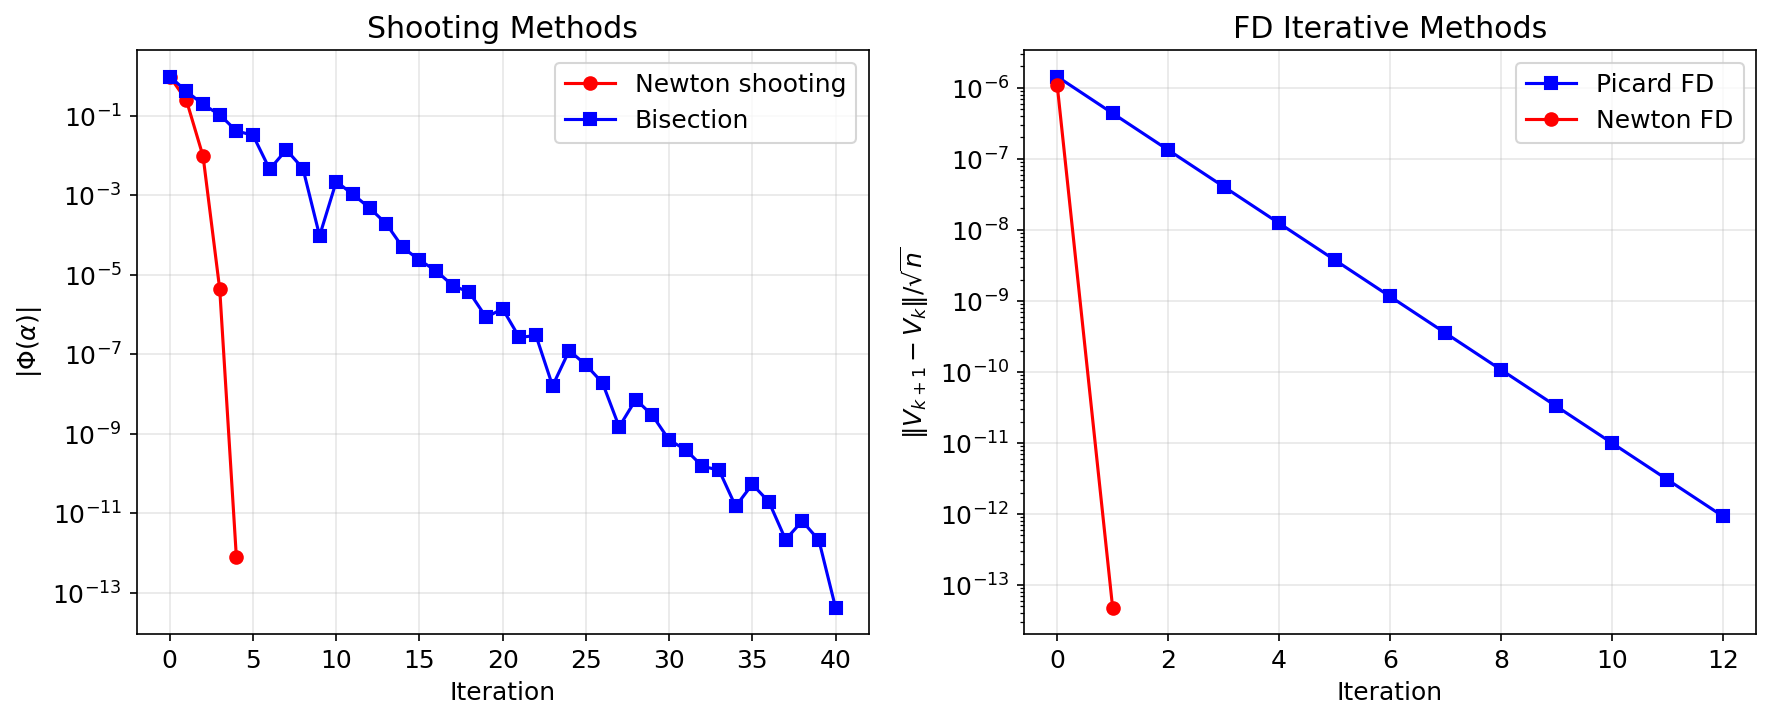
\includegraphics[width=\textwidth]{../code/Outputs/solvers_convergence.png}
\caption{Convergence histories of the four nonlinear solvers on Problem 3
         ($\beta = 0.1$, $n = 127$, tolerance $10^{-12}$). Left: shooting
         methods on $|\Phi(\alpha)|$, where Newton converges quadratically
         in 5 iterations and bisection linearly in 41.
         Right: FD iterations on the discrete residual, where Newton FD
         reaches the tolerance in 2 steps and Picard FD in 13.}
\label{fig:solvers}
\end{figure}


% ===========================================================================
\section{Physics-Informed Neural Networks as Nonlinear Collocation}
\label{sec:pinn}

PINNs are framed below as a nonlinear generalisation of classical
collocation, followed by the formulation, the hard-boundary-condition
ansatz, and the training recipe.


\subsection{Course Context: PINNs as Nonlinear Collocation}
\label{sec:collocation}

The Chapter 4 slides cover three projection-based approaches to BVPs:
\emph{collocation} \citep{khouider2026bvp}, \emph{Galerkin}, and
\emph{B-spline / FEM}. In classical linear collocation one picks a fixed
basis $\{\phi_k(x)\}_{k=1}^{M}$, writes the approximate solution as a
linear combination
\begin{equation}
\hat{u}(x) = \sum_{k=1}^{M} c_k \phi_k(x),
\label{eq:classical_coll}
\end{equation}
and enforces the PDE residual to be zero at $N_c$ collocation points
$\{x_j\}_{j=1}^{N_c}$. This produces a linear system in the coefficients
$c_k$ which can be solved directly.

PINNs are exactly this construction with the linear span of a fixed basis
replaced by the nonlinear function class represented by a neural network.
\Cref{tab:collocation_vs_pinn} summarises the correspondence.

\begin{table}[h]
\centering
\begin{tabular}{lll}
\toprule
 & \textbf{Linear collocation} & \textbf{PINN} \\
\midrule
Approximant       & $\sum c_k \phi_k(x)$        & neural network $\hat{u}(x;\theta)$ \\
Unknowns          & linear coefficients $c_k$   & network weights $\theta$  \\
Residual          & at $N_c$ collocation points & at $N_c$ collocation points \\
Solve method      & one linear system           & nonlinear optimisation \\
Mesh requirement  & structured basis            & any scattered points \\
Convergence       & provable (from basis theory) & no guarantee \\
\bottomrule
\end{tabular}
\caption{Correspondence between classical collocation and PINNs.}
\label{tab:collocation_vs_pinn}
\end{table}

\paragraph{Degrees of freedom.} One distinction that drives the
comparison plots in \cref{sec:acc_vs_n} is that the parameter count and
the sampling density are separate knobs in a PINN, whereas in FDM they
are the same quantity. For FDM, $n$ is simultaneously the grid size, the
number of unknowns, and the sampling density, and refining the grid
improves both resolution and representational capacity. For a PINN the
number of trainable weights is fixed by the architecture (roughly $3200$
for ours), and $N_c$ is the number of points at which the PDE residual is
evaluated. One can increase $N_c$ without changing the network, or enlarge
the network without adding collocation points. Sweeping $N_c$ therefore
answers the question \textit{does more sampling help a fixed model?}, which
is a genuinely different question from the one FDM refinement answers.


\subsection{Formulation}
\label{sec:pinn_form}

The PINN approximates the solution of the BVP by a neural network
$\text{NN}(x;\theta)$ with trainable parameters $\theta$. To ensure that
the boundary conditions are satisfied exactly at every training step
we use the hard-boundary-condition ansatz
\begin{equation}
\hat{u}(x;\theta) = g_0 (1 - x) + g_1 x + x (1 - x)\,\text{NN}(x;\theta),
\label{eq:hardbc}
\end{equation}
where $g_0 = u(0)$, $g_1 = u(1)$. The first two terms are the straight
line from $g_0$ to $g_1$ and already satisfy both boundary conditions; the
factor $x(1-x)$ in the third term vanishes at both endpoints, so the
network's contribution is zero on the boundary regardless of $\theta$. An
alternative is to add a soft penalty term to the loss for boundary
violations, but hard enforcement gives strictly better numerical behaviour
and removes a tunable weight from the loss.

For each problem the loss is the mean squared residual of the governing
equation at $N_c$ uniformly spaced interior collocation points
$\{x_j\}_{j=1}^{N_c}$:
\begin{equation}
\mathcal{L}(\theta) = \frac{1}{N_c} \sum_{j=1}^{N_c}
  \bigl| \mathcal{R}[\hat{u}](x_j;\theta) \bigr|^2,
\label{eq:loss}
\end{equation}
where $\mathcal{R}$ is the differential operator rearranged to have zero
on the right-hand side. For Problem 1, for instance,
$\mathcal{R}[\hat{u}] = \hat{u}'' + \pi^2 \sin(\pi x)$. The derivatives
$\hat{u}'$ and $\hat{u}''$ are computed via PyTorch's reverse-mode
automatic differentiation through the full expression in \cref{eq:hardbc},
which is exact up to floating-point arithmetic and does not incur any
discretisation error in the derivatives themselves. This is the sense
in which PINNs are mesh-free: neither the residual nor its derivatives
depend on a discretisation of space.

\paragraph{Why no analogue of the BVP convergence theorem exists.} For
FDM the error bound of \cref{sec:conv} follows from linearity and the
invertibility of $\Ah$: once the truncation error is controlled the
global error is controlled too. For a PINN the approximation is
nonlinear in $\theta$ and the error depends on the trajectory of a
non-convex optimiser. \citet{wang2022} analyse the PINN loss via its
neural tangent kernel and show that the residual and boundary loss terms
are driven at very different convergence rates under gradient descent, so
that one component can stall while the other continues to decrease.
\citet{rahaman2019} show that standard MLPs trained with gradient descent
exhibit a \emph{spectral bias} toward low-frequency components, so that
oscillatory features of the target solution are learned much more slowly
than smooth ones. \citet{wang2021eigenvector} make this diagnosis
PINN-specific and propose random Fourier-feature input embeddings
\citep{tancik2020} as one remedy.


\subsection{Architecture and Training}
\label{sec:pinn_train}

The architecture is fixed across all three problems and across all
values of $N_c$. \Cref{tab:pinn_arch} summarises it.

\begin{table}[h]
\centering
\begin{tabular}{ll}
\toprule
\textbf{Parameter} & \textbf{Value} \\
\midrule
Hidden layers       & 4 \\
Neurons per layer   & 32 \\
Activation          & $\tanh$ \\
Initialisation      & Xavier uniform, seed 42 \\
Trainable params    & $\approx 3200$ \\
\bottomrule
\end{tabular}
\caption{PINN architecture, held constant throughout the experiments.}
\label{tab:pinn_arch}
\end{table}

We use $\tanh$ rather than ReLU because the PDE residual
requires $\hat{u}''$ and ReLU is not twice differentiable.

\paragraph{Two-phase training.} Following \citet{raissi2019} we train in
two phases.
Phase 1 is 10{,}000 Adam steps at learning rate $10^{-3}$ with cosine
annealing, which brings the loss from its random initialisation down to
roughly $10^{-3}$. Phase 2 is a single \texttt{torch.optim.LBFGS} call
with strong Wolfe line search and up to 500 iterations, which polishes
the solution the rest of the way. In our runs the L-BFGS phase is
essential: without it the PINN error is roughly an order of magnitude
worse at every $N_c$. L-BFGS is a quasi-Newton method that approximates
the Hessian from the last few gradients, and it plays the same role here
as Newton FD plays in \cref{sec:picardnewton} (quadratic-ish
convergence once the iterate is close to a minimum).

\paragraph{Reproducibility.} All experiments use a fixed seed (42) for
NumPy, PyTorch, and weight initialisation. The PINN collocation points
are deterministic (uniform interior grid at each $N_c$). This makes the
runs deterministic modulo floating-point nondeterminism in CUDA; we run
everything on CPU.


\subsection{PINN Numerical Results}
\label{sec:pinn_results}

We train one PINN per problem per value of $N_c$, for
$N_c \in \{10, 25, 50, 100, 250, 500, 1000\}$, and record the final
$\Linf$ error, the final training loss, and the wall-clock time.
\Cref{tab:pinn_sweep} collects the accuracy numbers.

\begin{table}[h]
\centering
\small
\begin{tabular}{r|ccc}
\toprule
$N_c$ & \textbf{Problem 1} & \textbf{Problem 2} & \textbf{Problem 3} \\
\midrule
10    & $8.92 \times 10^{-5}$ & $1.76 \times 10^{-5}$ & $5.90 \times 10^{-5}$ \\
25    & $9.72 \times 10^{-6}$ & $1.87 \times 10^{-5}$ & $6.13 \times 10^{-5}$ \\
50    & $7.39 \times 10^{-6}$ & $2.03 \times 10^{-5}$ & $6.55 \times 10^{-5}$ \\
100   & $6.44 \times 10^{-6}$ & $2.17 \times 10^{-5}$ & $6.79 \times 10^{-5}$ \\
250   & $6.79 \times 10^{-6}$ & $2.15 \times 10^{-5}$ & $6.92 \times 10^{-5}$ \\
500   & $6.91 \times 10^{-6}$ & $2.23 \times 10^{-5}$ & $6.98 \times 10^{-5}$ \\
1000  & $6.44 \times 10^{-6}$ & $2.24 \times 10^{-5}$ & $7.07 \times 10^{-5}$ \\
\bottomrule
\end{tabular}
\caption{PINN $\Linf$ error versus number of collocation points. After an
         initial decrease for the smallest $N_c$ (Problem 1), the error
         is effectively constant in $N_c$ on all three problems.}
\label{tab:pinn_sweep}
\end{table}

The effective convergence rate between successive $N_c$ values is zero
for every problem beyond the smallest grids: increasing $N_c$ by an order
of magnitude does not reduce the error. On Problem 2 and Problem 3 the
error drifts slightly upward as $N_c$ grows, consistent with the
failure mode of \citet{wang2022}. The plateau is problem-dependent but
consistent across $N_c$: roughly $6 \times 10^{-6}$ for Problem 1,
$2 \times 10^{-5}$ for Problem 2, and $7 \times 10^{-5}$ for Problem 3.

\paragraph{Precision is not the cause.} An obvious candidate mechanism
for the plateau is that 32-bit floating-point accumulation in the PINN
residual prevents further progress. To rule this out, we re-ran the
entire PINN sweep in double precision
(\texttt{torch.set\_default\_dtype(torch.float64)}), keeping every other
hyperparameter identical. The plateau drops by at most a factor of two
(e.g.\ Problem 1 plateau moves from $\sim\!6.4 \times 10^{-6}$ to
$\sim\!3.1 \times 10^{-6}$, and Problem 2 is essentially unchanged at
$\sim\!3 \times 10^{-5}$), which is far smaller than the four orders of
magnitude of headroom that double precision provides. We conclude that
float32 arithmetic is not load-bearing on these problems and that the
plateau originates in the optimiser and the network's representational
dynamics, exactly as predicted by the references above.


% ===========================================================================
\section{Comparison}
\label{sec:comparison}

The two methods are now compared on the four axes of \cref{sec:intro}.


\subsection{Accuracy versus Sampling Density}
\label{sec:acc_vs_n}

\Cref{fig:accuracy} overlays the FDM and PINN accuracy sweeps on a
single log-log axis per problem. For FDM the horizontal axis is the
number of interior grid points $n$; for PINN it is the collocation
count $N_c$. As discussed in \cref{sec:collocation} these axes measure
different things, but both are the natural notion of \emph{sampling
density} for the respective method, and plotting them together makes
the qualitative difference immediate.

\begin{figure}[h]
\centering
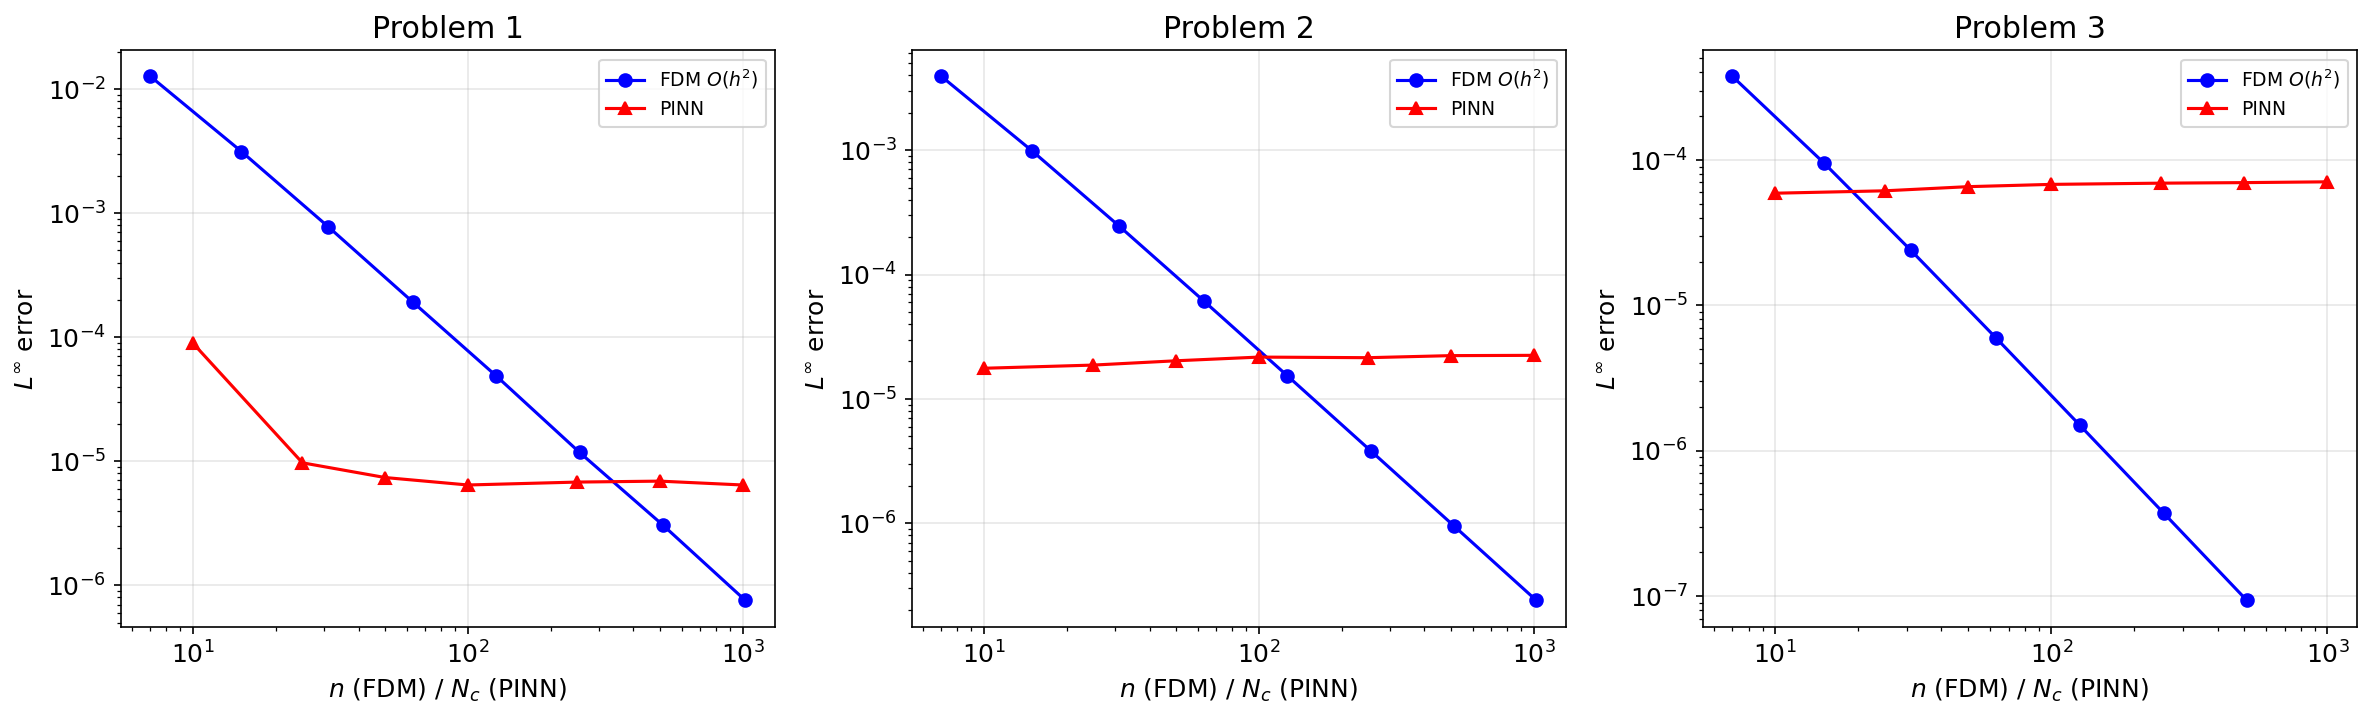
\includegraphics[width=\textwidth]{../code/Outputs/accuracy_vs_n.png}
\caption{FDM (blue) and PINN (red) $\Linf$ error versus sampling density
         (grid points $n$ for FDM, collocation points $N_c$ for PINN).
         FDM exhibits the theoretical slope $-2$ on all three problems
         and reaches sub-$10^{-6}$ accuracy by $n = 1023$.
         The PINN error plateaus around $6 \times 10^{-6}$ on Problem 1
         and around $2$ to $7 \times 10^{-5}$ on Problems 2 and 3,
         regardless of $N_c$.}
\label{fig:accuracy}
\end{figure}

FDM exhibits the straight-line slope $-2$ in log-log coordinates
predicted by \cref{sec:conv} and achieved numerically in
\cref{tab:fdm_conv}. PINN plateaus essentially instantly: after the
first doubling of $N_c$ the error is effectively flat. The two methods
cross at modest sampling density: on Problem 3, for example, FDM at
$n = 63$ already gives $5.97 \times 10^{-6}$, beating the PINN plateau
by an order of magnitude, and FDM at $n = 511$ outperforms the PINN by
nearly three orders of magnitude.


\subsection{Conditioning versus Loss Landscape}
\label{sec:cond_vs_loss}

Both methods have an accuracy ceiling, but the two ceilings have very
different character. \Cref{fig:cond_vs_loss} presents the two side by
side for Problem 1.

\begin{figure}[h]
\centering
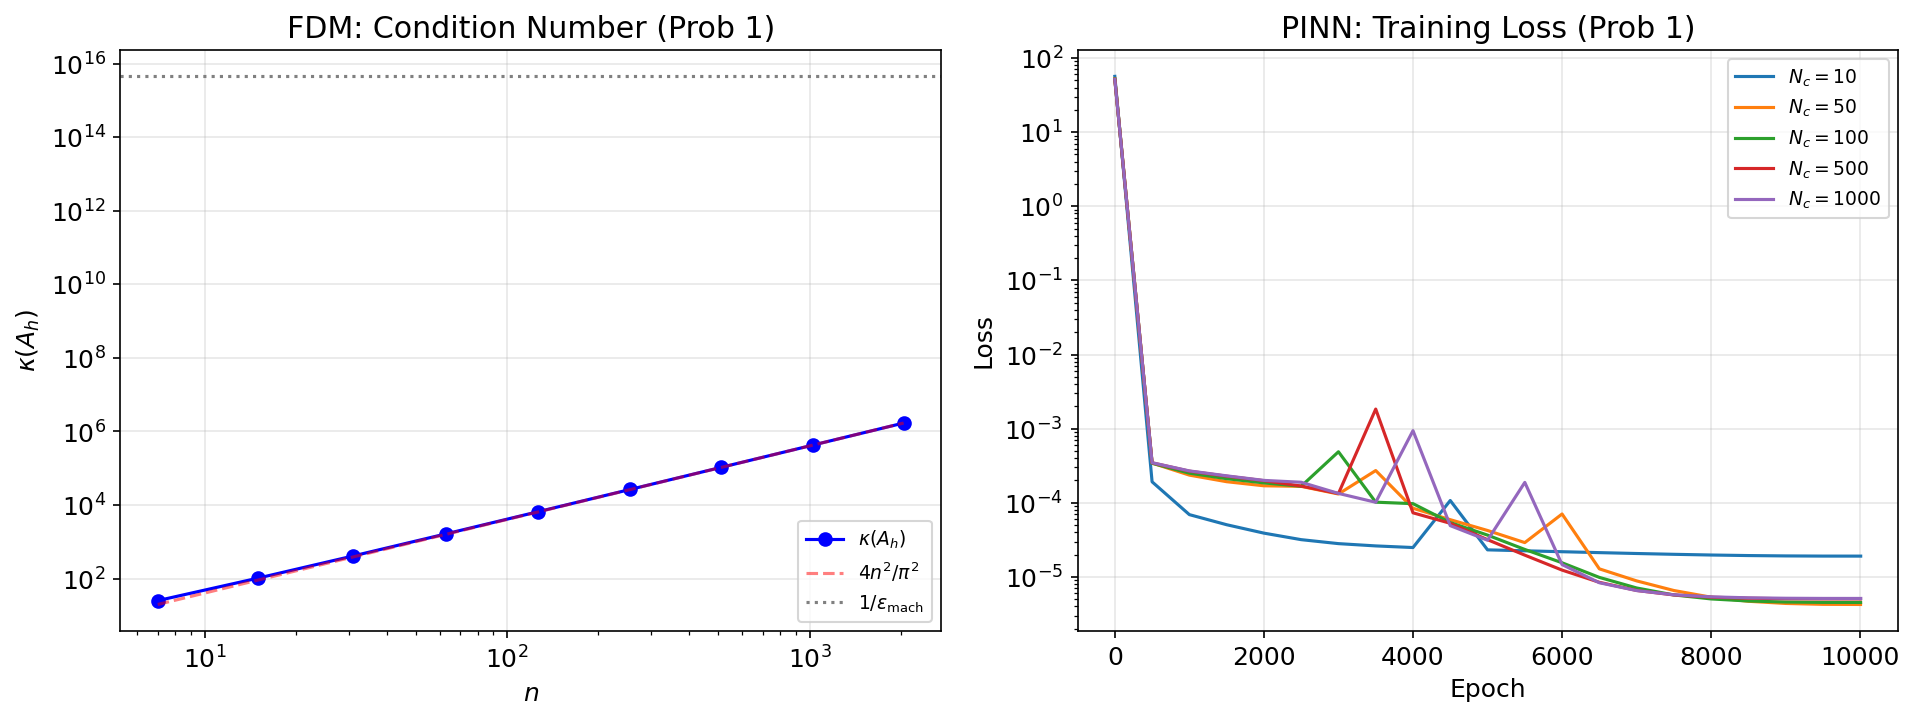
\includegraphics[width=\textwidth]{../code/Outputs/conditioning_vs_loss.png}
\caption{Two failure modes, same problem. Left: condition number
         $\kappa(\Ah)$ versus $n$ for the Problem 1 FDM matrix. The
         empirical curve (blue circles) matches the analytic
         $4(n+1)^2 / \pi^2$ (red dashed). The grey horizontal line is
         $1 / \epsilon_{\text{mach}}$ in double precision: FDM accuracy
         degrades once $\kappa \cdot \epsilon_{\text{mach}}$ approaches $1$.
         Right: PINN training loss versus epoch on Problem 1 for several
         values of $N_c$, showing a complicated but consistent descent
         to $\sim 10^{-7}$ regardless of $N_c$.}
\label{fig:cond_vs_loss}
\end{figure}

The FDM ceiling is analytic. From \cref{eq:cond} we know $\kappa(\Ah)$
exactly, and the empirical curve matches it; the threshold at which
linear-algebra roundoff overwhelms discretisation accuracy can be written
down before running any experiment. We do not reach this threshold in
our sweep: $\kappa(\Ah)$ at $n = 1023$ is $\sim 4 \times 10^5$, so the
worst-case amplification of double-precision roundoff is of order
$10^{-10}$, well below the $7.55 \times 10^{-7}$ discretisation error at
that grid.

The PINN ceiling is empirical. The training loss descends cleanly to
$\sim 10^{-7}$, but the test error plateaus at $\sim 10^{-5}$ to
$10^{-6}$: loss and error decouple. There is no theoretical prediction
for where this plateau sits; it must be measured after the fact.


\subsection{Iterative Solver Convergence Rates}
\label{sec:iter_conv}

\Cref{tab:iter_summary} puts all solvers used in the project on a single
page. The course hierarchy is exactly as predicted: linear-convergence
methods (bisection and Picard) need an order of magnitude more iterations
than quadratic-convergence methods (Newton shooting and Newton FD).
For comparison, the PINN is a quasi-Newton method (L-BFGS) on a
non-convex loss and requires on the order of $10^4$ iterations to
reach its plateau.

\begin{table}[h]
\centering
\begin{tabular}{lll}
\toprule
\textbf{Solver} & \textbf{Asymptotic rate} & \textbf{Iterations to $10^{-12}$ (Prob 3)} \\
\midrule
Bisection shooting   & linear     & 41 \\
Newton shooting      & quadratic  & 5 \\
Picard FD            & linear     & 13 \\
Newton FD            & quadratic  & 2 \\
PINN (Adam + L-BFGS) & non-convex & $\sim 10^{4}$ (plateau only) \\
\bottomrule
\end{tabular}
\caption{Summary of iterative solvers used in the project. The first
         four are the classical course methods, applied to Problem 3.
         The last row is the PINN optimiser, included for perspective.}
\label{tab:iter_summary}
\end{table}


\subsection{Computational Cost}
\label{sec:cost}

The wall-clock costs of the two methods differ by roughly five orders
of magnitude. \Cref{tab:timing} reports representative numbers.

\begin{table}[h]
\centering
\begin{tabular}{lr}
\toprule
\textbf{Method} & \textbf{Wall-clock time} \\
\midrule
FDM, Problem 1, $n = 63$      & $\approx 210 \mu s$ \\
FDM, Problem 1, $n = 255$     & $\approx 200 \mu s$ \\
FDM, Problem 1, $n = 1023$    & $\approx 370 \mu s$ \\
FDM, Problem 3, $n = 255$     & $\approx 1.2 ms$ \\
PINN, Problem 1, $N_c = 100$, training & $\approx 16 s$ \\
PINN, Problem 1, $N_c = 1000$, training & $\approx 74 s$ \\
PINN inference (any problem) & $\approx 400 \mu s$ \\
\bottomrule
\end{tabular}
\caption{Representative wall-clock times on CPU. FDM includes the full
         tridiagonal solve; PINN training includes 10k Adam steps and
         the L-BFGS refinement; PINN inference is a forward pass on
         1000 test points from an already-trained model.}
\label{tab:timing}
\end{table}

At the accuracy the PINN achieves ($\sim 10^{-5}$), FDM delivers the
same accuracy at $n \le 63$ in a few hundred microseconds, making the
training-cost ratio roughly $10^5$ against the PINN. PINN inference
(400 microseconds, once trained) is essentially equal to the FDM solve
time; the mesh-free evaluation does not help a 1D problem where the
mesh is trivial to build.


% ===========================================================================
\section{Conclusions}
\label{sec:conclusions}

Across all three test problems and on every axis we measured, the classical
finite difference method is strictly better than the PINN for the class of
problems under consideration:

\begin{itemize}
\item \textbf{Accuracy} is higher for FDM at every sampling density we
      tested beyond the smallest grids, with a clean second-order scaling
      that takes FDM below $10^{-6}$ at $n = 1023$. The PINN plateau
      sits at $\sim\!10^{-5}$ on Problems 2 and 3 independent of $N_c$.
\item \textbf{The failure mode is theoretically characterised} for FDM
      (condition-number-limited roundoff, reachable only at very fine
      grids), whereas the PINN plateau is empirical and not
      predictable from first principles; we verified that it is not a
      precision artefact.
\item \textbf{Iterative convergence} on the nonlinear problem follows
      the course hierarchy exactly: quadratic methods (Newton shooting,
      Newton FD) dominate linear ones (bisection, Picard), and both are
      orders of magnitude faster to converge than the PINN optimiser.
\item \textbf{Wall-clock cost} is roughly five orders of magnitude lower
      for FDM than for PINN training at the accuracy level the PINN
      actually achieves.
\end{itemize}

PINNs are not a drop-in replacement for classical numerical methods on
problems where the classical methods already have complete theory. The
settings where PINNs may be preferable are those where FDM is awkward
or impossible: inverse problems, where \citet{raissi2019} demonstrate
that PINNs can jointly recover the solution and unknown PDE parameters
from sparse noisy data, and problems on irregular or high-dimensional
domains where mesh generation becomes the bottleneck.


% ===========================================================================
\section{Further Research}
\label{sec:further}

Within the scope of the comparison itself, several extensions were
planned but not executed in time for this submission. Each is documented
here so that the gaps in the experimental story are explicit, and to
record the state of the partial implementations that exist in the
project repository.

\paragraph{Random Fourier-feature input embedding.} Of the candidate
mechanisms for the PINN accuracy plateau, the experiment in
\cref{sec:pinn_results} rules out floating-point precision and leaves
spectral bias and the non-convex optimisation landscape as the
remaining candidates. The cleanest test of the spectral-bias hypothesis
is to prepend a random Fourier-feature input embedding
\citep{tancik2020,wang2021eigenvector} to the network. The embedding
\begin{equation*}
\gamma(x) = \bigl[ \sin(2 \pi B x),\ \cos(2 \pi B x) \bigr],
\quad B_i \sim \mathcal{N}(0, \sigma^2),
\end{equation*}
is sampled once at initialisation and held fixed; the network is then
trained on $\gamma(x)$ rather than on $x$ directly. If spectral bias is
load-bearing, the Fourier-embedded PINN should reach a smaller plateau
on Problem 1 (whose exact solution $\sin(\pi x)$ has obvious frequency
content) than the baseline does. If the plateau is unchanged across
problems, spectral bias is also ruled out and the remaining mechanism
is non-convexity of the loss landscape. The notebook
\texttt{code/main\_fourier.ipynb} contains the full implementation, a
two-stage sweep (a $\sigma$ pilot at $N_c = 100$ followed by a full
$N_c$ sweep at the per-problem winning $\sigma$), and the analysis
plots; only the actual training runs were not completed in time.
Other architectural and training-recipe modifications (loss reweighting,
longer L-BFGS phases, adaptive collocation sampling) could be tested in
the same framework.

\paragraph{Higher-order FDM via Richardson extrapolation.} On the
classical side, the natural follow-up is to increase the order of the
FDM accuracy via Richardson extrapolation. The extrapolated solution
$u_{\text{rich}} = (4\,u_{h/2} - u_h)/3$ cancels the leading $\bigO(h^2)$
error term and yields $\bigO(h^4)$ accuracy with no additional stencil
work, which would push FDM well past its current advantage and reach
the condition-number ceiling at much smaller $n$. This is a one-line
change on top of the existing FDM solver and would extend
\cref{tab:fdm_conv} with two more columns; it was deferred because the
existing comparison already establishes the qualitative result.

\paragraph{Higher dimensions and irregular geometries.} The most
plausible setting in which PINNs could outperform FDM is in dimensions
where mesh generation becomes expensive or the curse of dimensionality
makes a regular grid impractical. A natural next experiment would be
the same comparison on the 2D Poisson equation on an L-shaped domain,
where the corner singularity and the non-rectangular boundary make
classical methods awkward and where mesh-free residual sampling is at
its most attractive. Conversely, extending FDM to 2D would require
either a five-point Laplacian on a Cartesian grid (clean but inflexible)
or a finite element discretisation, which is out of scope for this
course.

\paragraph{Inverse problems.} The clearest practical advantage of
PINNs documented in the original \citet{raissi2019} paper is the inverse
setting: given sparse noisy observations of a solution, recover both
the solution and unknown parameters of the governing equation. There is
no analogue of this for FDM, which solves only forward problems with
known coefficients. A test problem would be Problem 2 with the
coefficient $a(x) = 1 + x^2$ replaced by an unknown $a(x)$ to be
recovered jointly with $u$ from a handful of interior measurements.
This is a qualitatively different experiment from the comparison done
here and would require a separate paper.


% ===========================================================================
\bibliographystyle{plainnat}
\bibliography{refs}

\end{document}
